\documentclass[11pt]{amsart}

\usepackage{amssymb}
\usepackage{amsthm}
\usepackage{amsmath}

%\usepackage[margin=1in]{geometry}

\usepackage[usenames]{color}
\usepackage{tikz}

\usepackage{hyperref}

\theoremstyle{plain}
\newtheorem{proposition}{Proposition}[section]
\newtheorem{theorem}[proposition]{Theorem}
\newtheorem{lemma}[proposition]{Lemma}
\newtheorem{corollary}[proposition]{Corollary}
\theoremstyle{definition}
\newtheorem{example}[proposition]{Example}
\newtheorem{definition}[proposition]{Definition}
\newtheorem{observation}[proposition]{Observation}
\theoremstyle{remark}
\newtheorem{remark}[proposition]{Remark}
\newtheorem{conjecture}[proposition]{Conjecture}
\newtheorem{question}[proposition]{Question}
\newtheorem{problem}[proposition]{Problem}


\DeclareMathOperator{\id}{id}

\DeclareMathOperator{\dist}{d}
\DeclareMathOperator{\CAT}{\mathsf{CAT}}
\DeclareMathOperator{\Isom}{\mathsf{Isom}}
\DeclareMathOperator{\PSL}{\mathsf{PSL}}
\DeclareMathOperator{\SL}{\mathsf{SL}}


%%%%%%%%%%%%%%%%%%%%%%%%%%%%%%%%%%%%%%%%%%%%%%%%%%%%%%%%%%%%%%%%%%%%%%%%%%%%%%%%%%%%%%%%%%%%%%%%%%%%%%%%%%%%%%%%%

\newcounter{countharry}
\setcounter{countharry}{1}
\newcommand{\comharry}[1]{{\textcolor{red}{\textrm{{\bf (\arabic{countharry})\stepcounter{countharry} Harry:} #1}}}}


\newcounter{countchenxi}
\setcounter{countchenxi}{1}
\newcommand{\comchenxi}[1]{{\textcolor{blue}{\textrm{{\bf
(\arabic{countchenxi})\stepcounter{countchenxi} Chenxi:} #1}}}}


%%%%%%%%%%%%%%%%%%%%%%%%%%%%%%%%%%%%%%%%%%%%%%%%%%%%%%%%%%%%%%%%%%%%%%%%%%%%%%%%%%%%%%%%%%%%%%%%%%%%%%%%%%%%%%%%

\date{\today}

\begin{document}

\title{
  A 0-1 law and cusp excursion for geometrically finite actions on coarsely
  hyperbolic metric spaces
}
\author{Harrison Bray}
%\address{.}
%\email{}
\date{\today}
\keywords{}
\subjclass[2020]{}

\begin{abstract} 
  Based on joint work with Giulio Tiozzo.
\end{abstract}

\maketitle

\tableofcontents

\section{Introduction}


Given a function $\psi\colon\mathbb N\to \mathbb R+$, define
\[ 
  \Theta(\psi)=\{x\in\mathbb [0,1] : |x-\frac{p}q|<\frac{\psi(q)}q
  \text{ for infinitely many reduced rationals }\frac{p}q \}
\]

\begin{theorem}[Khinchin, 1926]
  Let $\psi\colon \mathbb N\to\mathbb R^+$ be monotone decreasing.
  \comharry{is this even needed? any other hypotheses?}
  Then 
  \[
    \sum_{q\in\mathbb R} \psi(q)=\infty \; \text{ then }\; \Theta(\psi)
    \text{ has measure 1}
  \]
  and 
  \[
    \sum_{q\in\mathbb R} \psi(q)=0 \; \text{ then }\; \Theta(\psi)
    \text{ has measure zero}.
  \]
  \label{thm:khinchin}
\end{theorem}

Thus, Theorem~\ref{thm:khinchin} is a strong 0-1 law for the interval. As
an application, we have the following classical example: 

\begin{example}
  Let $\psi_\epsilon(q)=q^{-(1+\epsilon)}$. Then 
  \[
    \Theta(\psi_\epsilon)=\{
      x\in\mathbb R :
      |x-\frac{p}q|<\frac1{q^{2+\epsilon}}
      \text{ 
	for infinitely many
      }\frac{p}q\in\mathbb Q
    \}.
  \]
  Let us illustrate the limsup set $\Theta(\psi_0)$. 

  \begin{figure}[h!]
    \centering
        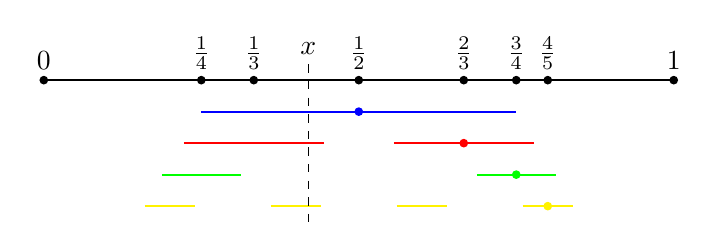
\begin{tikzpicture}[scale=8,thick]
    \draw[-] (0,0)--(1,0); 
    \def\s{.005}

    \def\e{.05}
    \draw[blue] (.25,-\e)--(.75,-\e);
    \draw[fill,blue] (.5,-\e) circle (\s) node {};


    \begin{scope}[red]
      \draw[] (.555555,-2*\e)--(.77777,-2*\e);
      \draw[] (.33333-.111111,-2*\e)--(.333333+.111111,-2*\e);
      \draw[fill] (.6666667,-2*\e) circle (\s) node {};
    \end{scope}

    \begin{scope}[green]
    \draw[] (.6875,-3*\e)--(.8125,-3*\e);
    \draw[fill] (.75,-3*\e) circle (\s) node {};

    \draw[] (.25-0.0625,-3*\e)--(.25+0.0625,-3*\e);
    \end{scope}


    \begin{scope}[yellow]
      
    \draw[] (.76,-4*\e)--(.84,-4*\e);
    \draw[fill] (.8,-4*\e) circle (\s) node {};

    \draw[] (.2-.04,-4*\e)--(.2+.04,-4*\e);
    \draw[] (.4-.04,-4*\e)--(.4+.04,-4*\e);
    \draw[] (.6-.04,-4*\e)--(.6+.04,-4*\e);

    \end{scope}

    \draw[fill] (0,0) circle (\s) node[above] {$0$};
    \draw[fill] (1,0) circle (\s) node[above] {$1$};
    \draw[fill] (.25,0) circle (\s) node[above] {$\frac14$};
    \draw[fill] (.33333,0) circle (\s) node[above] {$\frac13$};
    \draw[fill] (.5,0) circle (\s) node[above] {$\frac12$};
    \draw[fill] (.666667,0) circle (\s) node[above] {$\frac23$};
    \draw[fill] (.75,0) circle (\s) node[above] {$\frac34$};
    \draw[fill] (.8,0) circle (\s) node[above] {$\frac45$};


    \draw[dashed,thin] (.42,.5*\e) node[above] {$x$} -- (.42,-4.5*\e);
  \end{tikzpicture}

    \caption{
      An illustration of the first levels of the limsup set
      $\Theta(\psi_0)$. The intervals around $\frac12$ have radius $\frac14$,
      around $\frac23$ have radius $\frac19$, and so on.
    }
    \label{fig:khinchin}
  \end{figure}

  See that 
  \[
    \sum_{q\in\mathbb N}\psi_\epsilon(q)=\sum_{q\in\mathbb
    N}\frac1{q^{1+\epsilon}}
     \left\{
      \begin{array}[]{cc}
	=\infty & \text{ for }\epsilon=0\\
	<\infty & \text{ for }\epsilon>0
      \end{array}
    \right.
  \]
  hence
  Khinchin's theorem implies 

  \[
    \Theta(\psi_\epsilon) \text{ has measure }
    \left\{
      \begin{array}[]{l}
	\text{  one for }\epsilon=0 \\
	\text{  zero for }\epsilon>0.
      \end{array}
    \right.
  \]

  Thus in Figure~\ref{fig:khinchin}, $x$ is in infinitely many balls of radius
  $\frac1{q^2}$ about $\frac{p}q$ with probability 1. 

\end{example}

We will now discuss an analogy of Khinchin's Theorem (\ref{thm:khinchin})
for the hyperbolic plane, due originally to Sullivan \cite{sullivan84}.


\subsection{Horoball packings for the hyperbolic plane} 

The results of Sullivan generalize but we present them for surfaces, or
really for a particular surface, to communicate the concept. A statement
in full generality appears \comharry{ref} and is the goal of these notes. 

Recall a { \em  Fuchsian group} is a discrete subgroup $\Gamma$ of $\PSL(2,\mathbb
R)$, which acts on the upper half-plane model of hyperbolic 2-space
$\mathbb H^2$ by isometries via M\"obius transformations. Let
$\Sigma_{g,n}$ denote a surfaces of genus $g$ with $n$ punctures. Consider a
representation $\Gamma<\PSL(2,\mathbb R)$ of $\pi_1(\Sigma_{0,1})$ which
acts cofinitely on $\mathbb H^2$; that is, the quotient $\mathbb
H^2/\Gamma$ has finite area. 










\bibliographystyle{plain}
\bibliography{refs}


\end{document}



